
\chapter{cuDPP}
\label{chap:cudpp}

\section{Introduction}
\label{sec:introduction-5}

\begin{framed}
  cuDPP (so far at version 1.1) only work at the level of CUDA C
  runtime APIs.
\end{framed}

CUDA Data Primitive Parallel (cuDPP) is a library that supports
parallel reduction, segmentation scan (prefix sum), sort... It is the
result of the collaboration between UC, Davis and NVIDIA. cuDPP
provides similar functionality to \hyperref[chap:thrust]{Thrust}. The
essential difference is that {\it cuDPP interfaces is designed for
performance, while Thrust interface is designed for productivity.}

cuDPP provide a pre-compiled library that can be linked to any codes
written in C/Fortran (thanks to new interoperability of Fortran
2003). Yet Thrust need to be compiled first with \verb!nvcc! before it
can be linked to any other programs (Sect.~\ref{sec:building-cudpp}).

To work with CUDA 3.0, we need cuDPP 1.1.1. For more information, read
Sect.~\ref{sec:cudpp-1}. 

{\bf IMPORTANT}: cuDPP doesn't handle allocation or data
transfers. So, all data given to cuDPP routines must resides on GPU;
and user need to manually copy the result back to CPU, if necessary. 

Important concepts:
\begin{enumerate}
\item {\bf reduction}: Many parallel threads need to generate a single
  result value, e.g. min/max... Fig.~\ref{fig:reduction}
\begin{figure}[hbt]
  \centerline{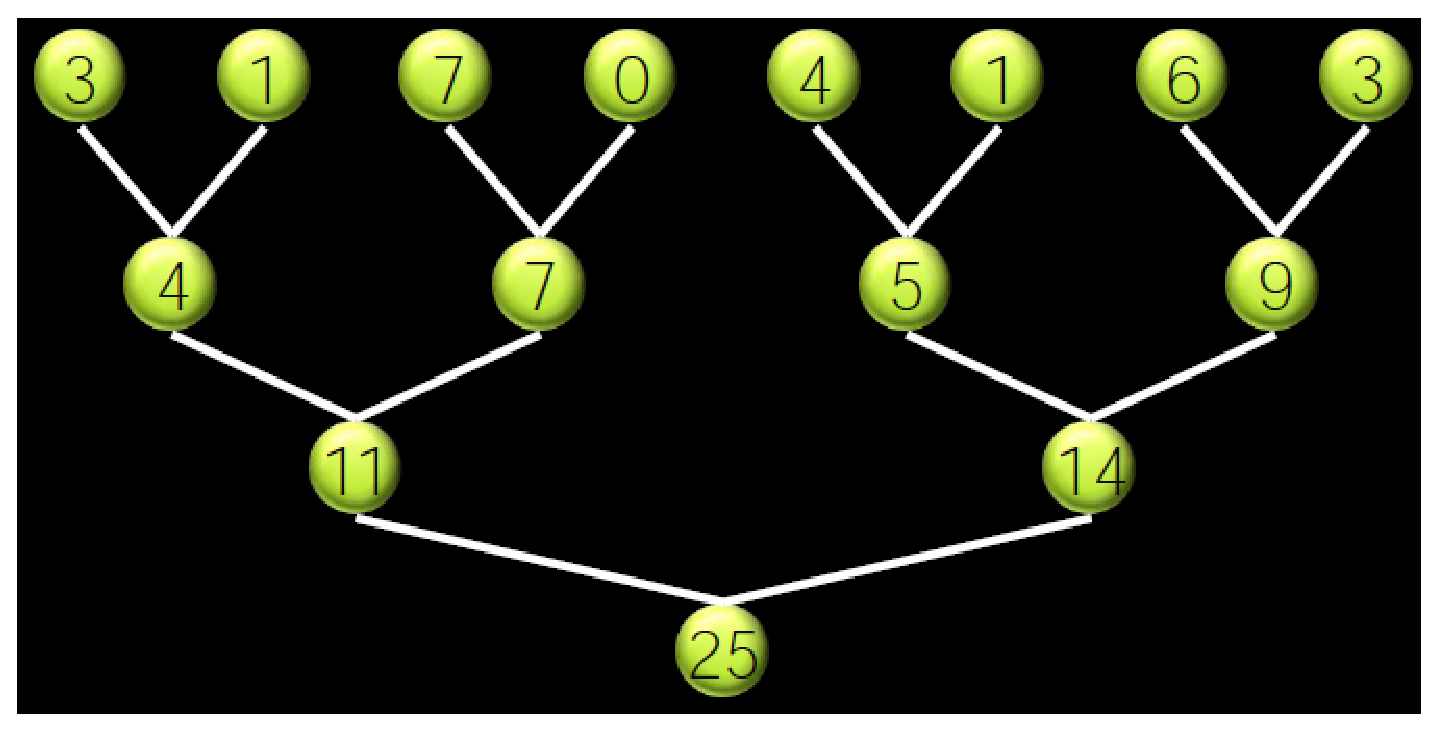
\includegraphics[height=3cm,
    angle=0]{./images/reduction.eps}}
  \caption{Tree-based implementation of reduction}
\label{fig:reduction}
\end{figure}

\item {\bf split}: Many parallel threads need to partition data,
  e.g. sorting, building tree. Fig.~\ref{fig:split}
\begin{figure}[hbt]
  \centerline{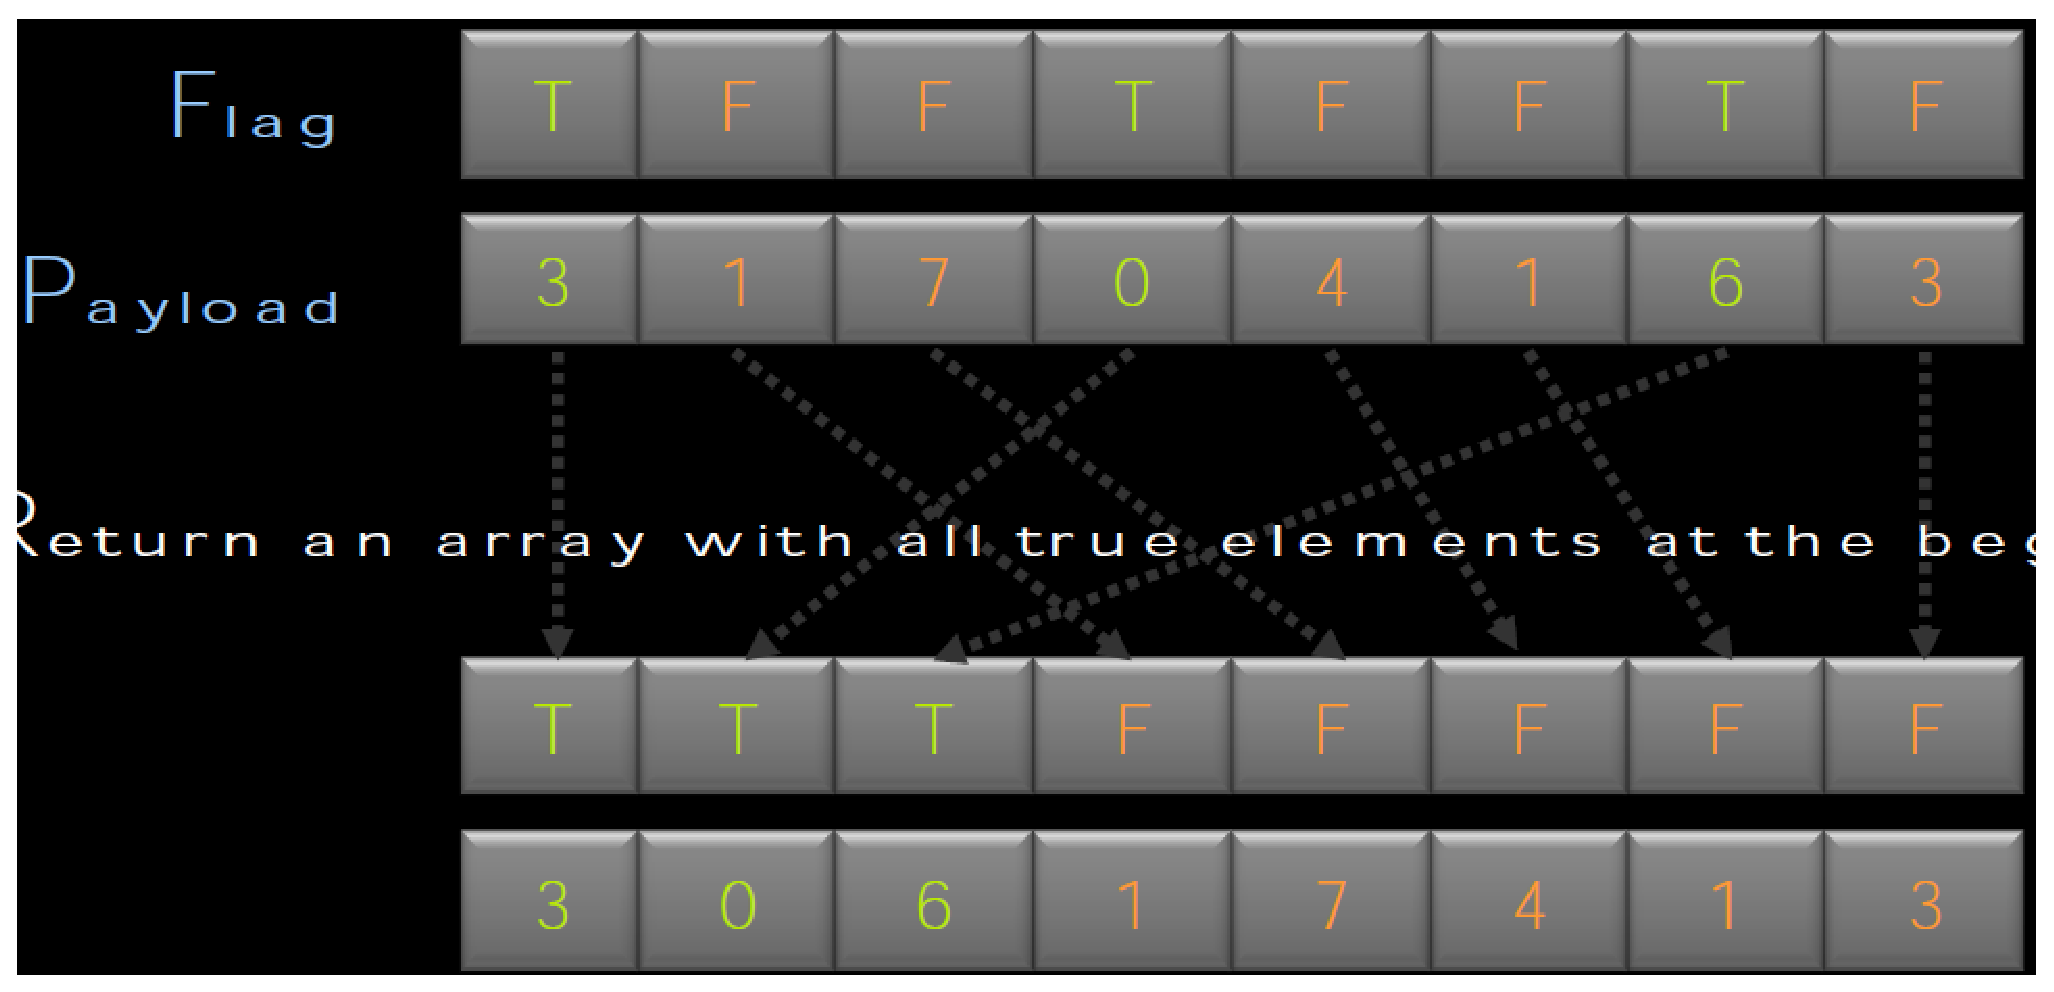
\includegraphics[height=3cm,
    angle=0]{./images/split.eps}}
\caption{Sorting data}
\label{fig:split}
\end{figure}

\item {\bf compact/expand/allocate}: Many parallel threads have
  variable output per threads, e.g. collision (e.g. remove zero
  elements) Fig.~\ref{fig:compact}, variable storage detection
  (e.g. marching cubes, geometry generation)
  Fig.~\ref{fig:variable_storage}.
\begin{figure}[hbt]
  \centerline{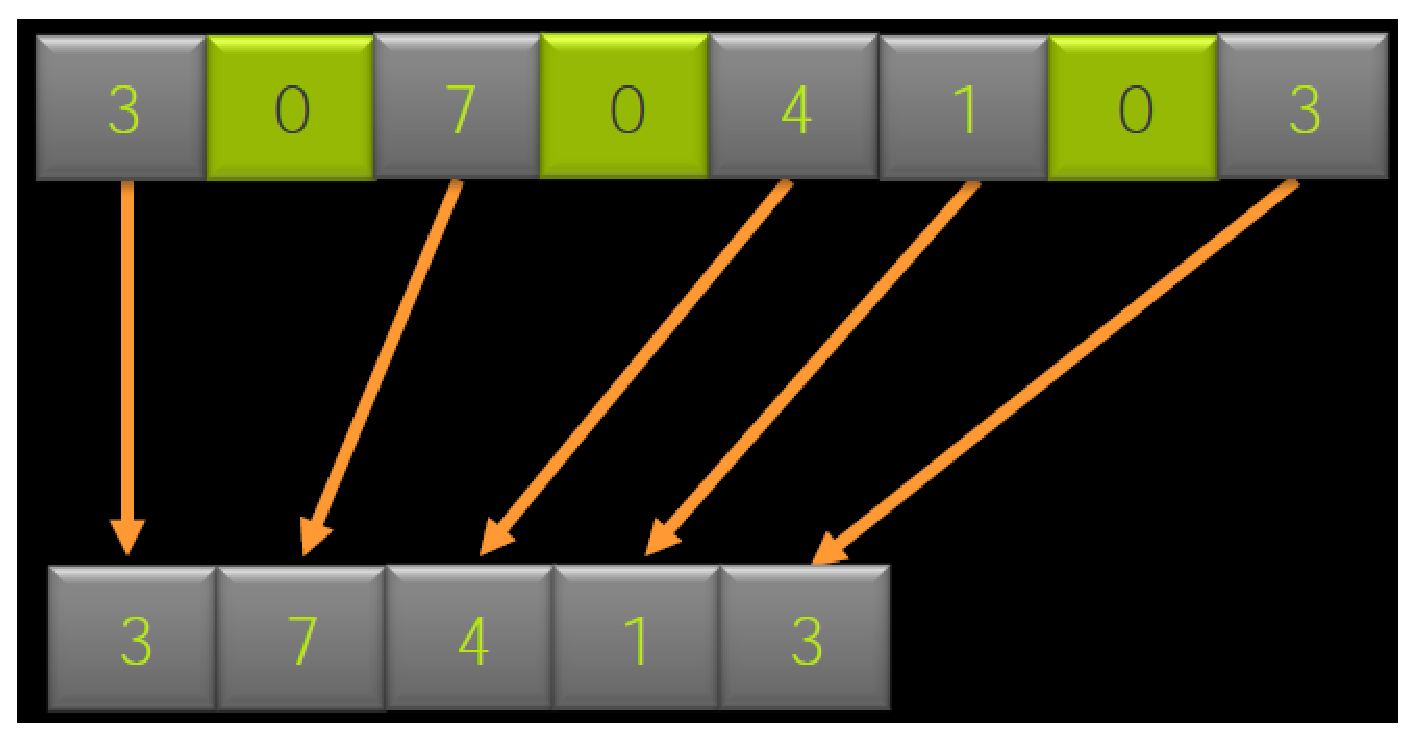
\includegraphics[height=3.4cm,
    angle=0]{./images/compact.eps}}
  \caption{Parallel the removing of zero elements}
\label{fig:compact}
\end{figure}

\begin{figure}[hbt]
  \centerline{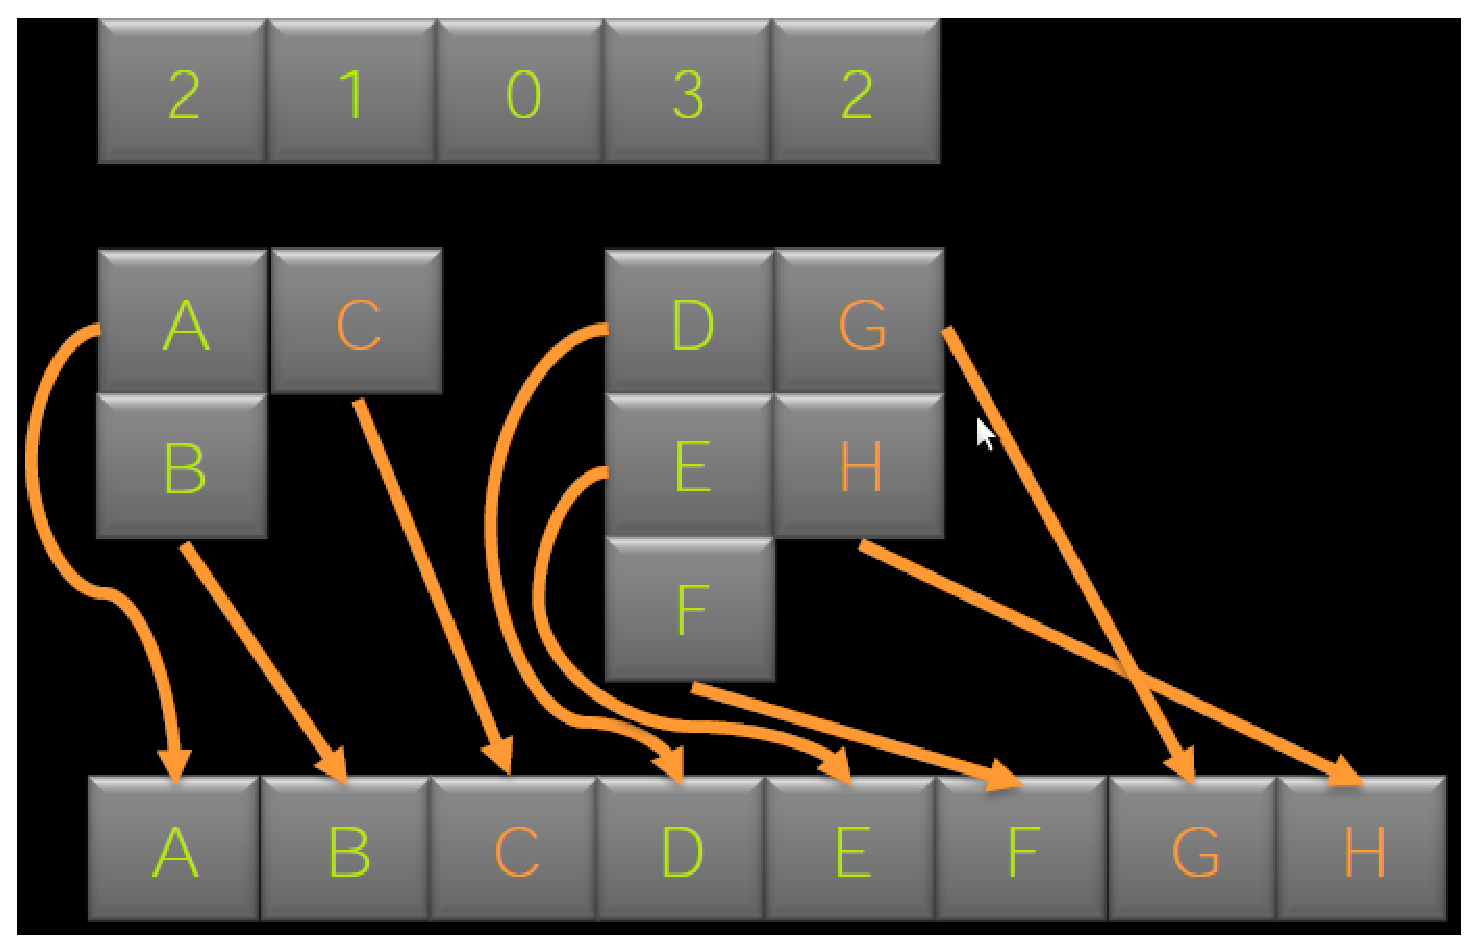
\includegraphics[height=4cm,
    angle=0]{./images/variable_storage.eps}}
 \caption{Different threads have different amounts of data}
\label{fig:variable_storage}
\end{figure}

\item {\bf scan}: suppose ``scan'' is an operator $\oplus$ with
  identity $\kappa$. Then, for an array $A=(a_1,a_2,\dots,a_n)$, when
  the scan operator is applied, we get the result 
  \begin{eqnarray}
    \label{eq:1}
    A = \left( \kappa, (a_1\oplus a_2),\dots, (a_1\oplus a_2\oplus \dots
    \oplus a_n)\right)
  \end{eqnarray}
Example: ``scan'' is addition. 
\begin{verbatim}
[3 1 7 0 4 1 6 3]
return
[0 3 4 11 11 15 16 22]
\end{verbatim}

\end{enumerate}

A similar library is Thrust (read Chap.~\ref{chap:cufft}). 
References:
\begin{itemize}
\item \url{http://www.gpgpu.org/developer/cudpp}
\item \url{http://code.google.com/p/cudpp}
\item \url{http://code.google.com/p/thrust/wiki/ThrustAndCUDPP}
\item \url{http://cudpp.googlecode.com/svn/tags/1.1.1/cudpp/doc/html/index.html}
\end{itemize}


\section{Scan}
\label{sec:scan}

Scan is the primitive operation in almost all parallel operations
\begin{enumerate}
\item radix
  sort\footnote{\url{http://mgarland.org/papers.html}}\citep{satish2009des}
  - implemented on cuDPP as \verb!cudppSort()!. This is faster than
  merge sort. 
\item quicksort (segmented scan - divide into partitions that enable
  parallel quicksort and parallel sparse matrix-vector multiply in CSR
  format) 
\begin{figure}[hbt]
  \centerline{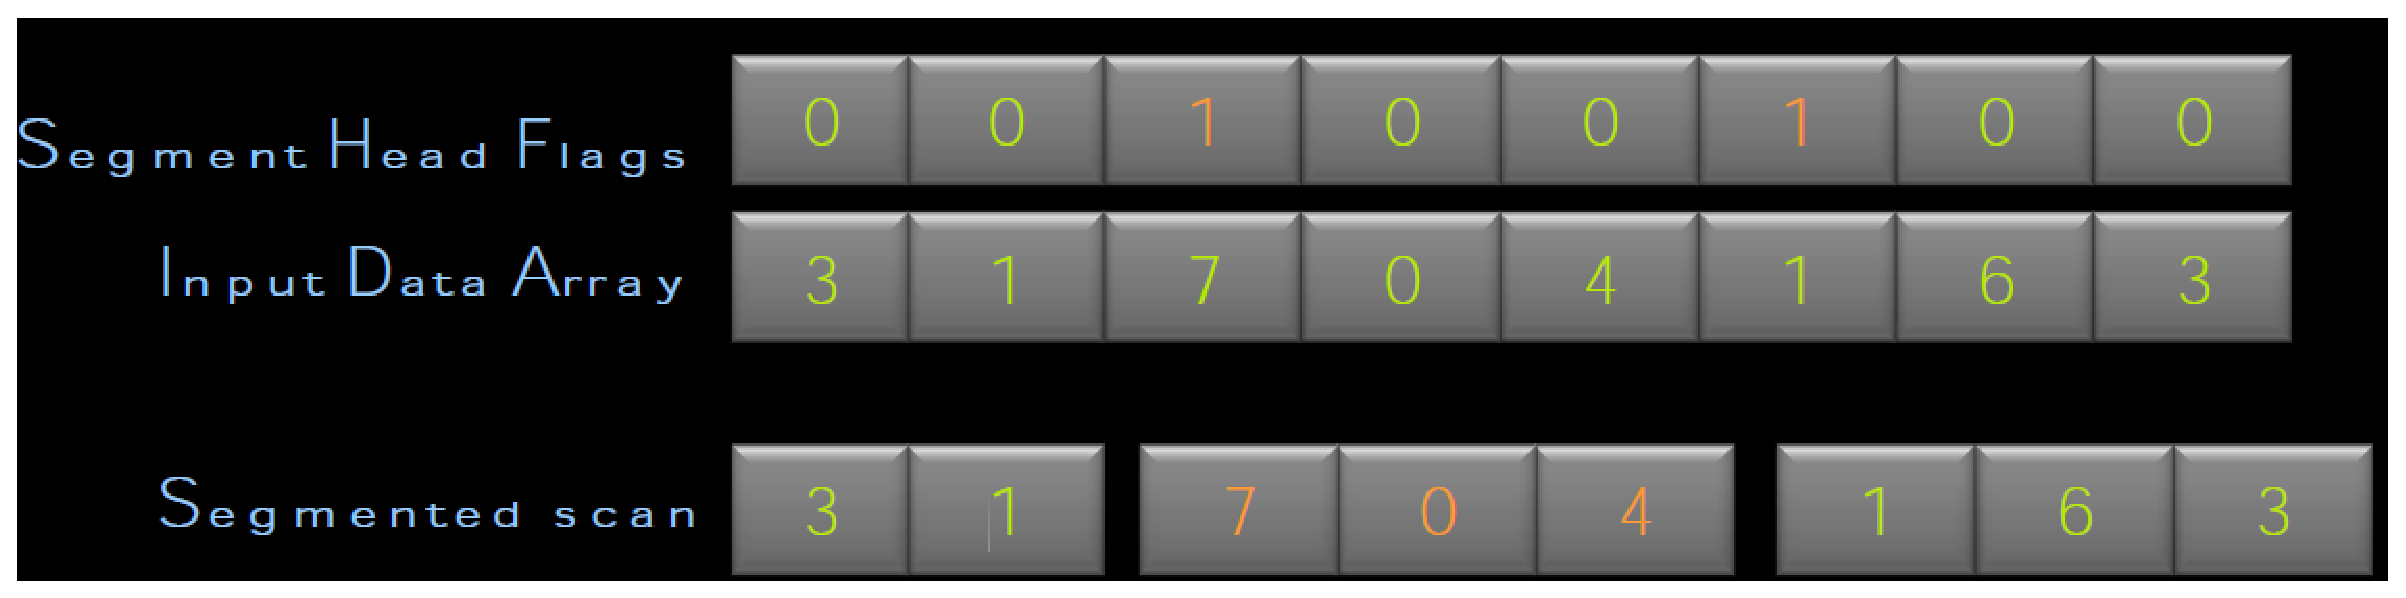
\includegraphics[height=2cm,
    angle=0]{./images/segmented_scan.eps}}
\caption{Segmented scan}
\label{fig:segmented_scan}
\end{figure}

\item String comparison
\item Lexical analysis
\item Stream compaction, i.e. retain certain elements only
  {\bf Example}: Parallel prefix sum (scan) in
  CUDA\citep{harris2010pps}. The grey value can be selected by building a
  scan sum, then choosing the end value of each team in the scan sum,
  as shown in Fig.~\ref{fig:stream_compaction}.
\begin{figure}[hbt]
  \centerline{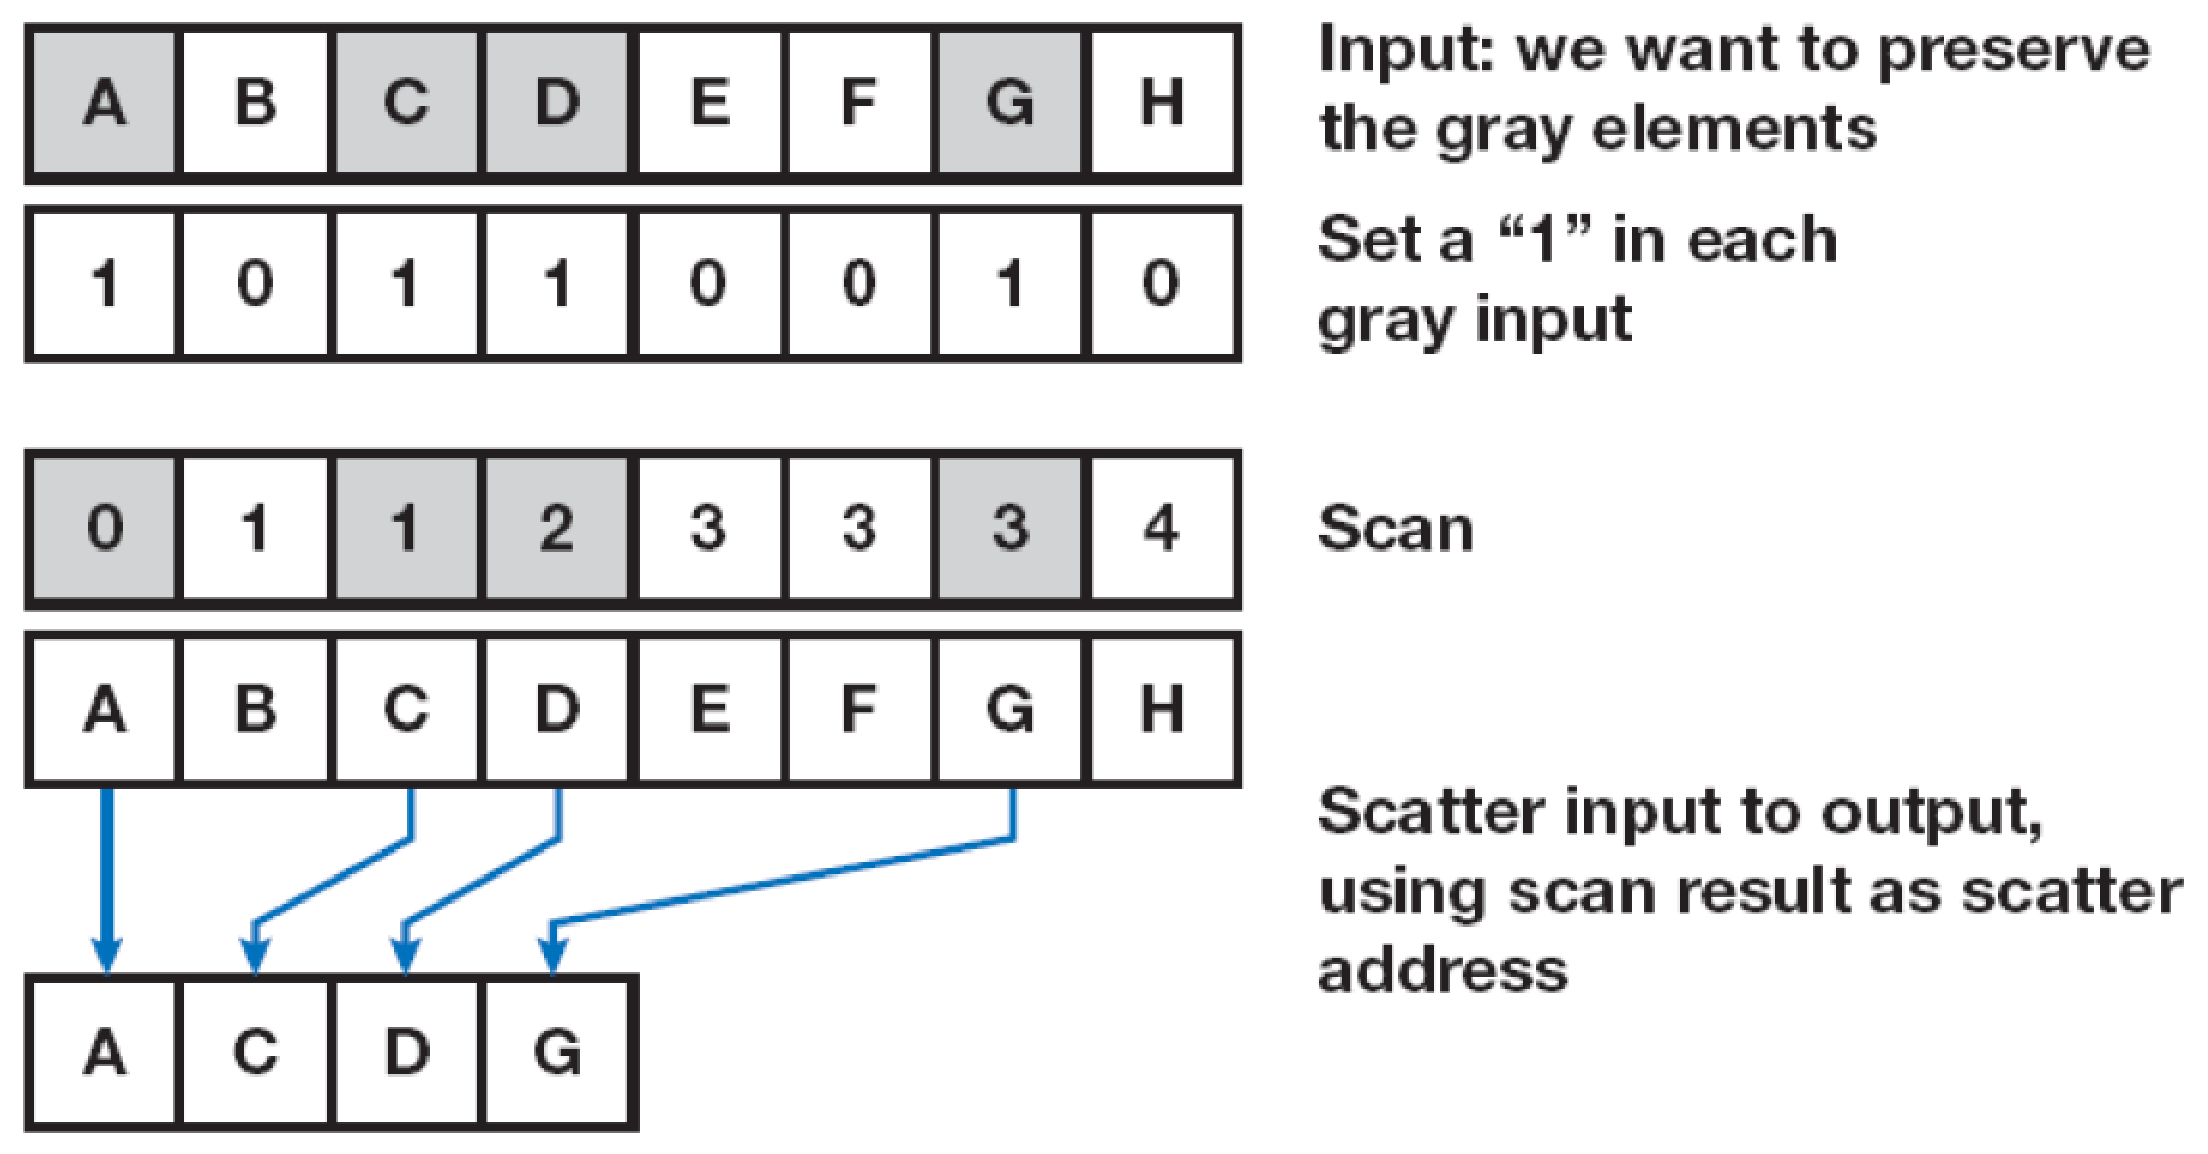
\includegraphics[height=5cm,
    angle=0]{./images/stream_compaction.eps}}
\caption{Select some values based on certain condition}
\label{fig:stream_compaction}
\end{figure}

\item Run-length encoding
\item Polynomial evaluation
\item Solving recurrences
\item Tree operations
\item Histograms
\item Allocation
\item ...
\end{enumerate}
Surprisingly, scan is unnecessary operation in sequential
computing. The history of using ``scan'' operation is given
\begin{itemize}
\item Pre-GPU
\begin {enumerate}
\item Iverson (1962) first proposed ``scan'' operator in APL
  programming language
\item In 1990, it's a feature of C* and CM-Lisp, i.e. a data primitive
  structure in Connection Machine
\item Guy Blelloch (1990) has a paper imposing the importance of scan
  operator ``Prefix sum and their applications''. 
\end{enumerate}
\item Post-GPU
  \begin{enumerate}
  \item GPU implementation of ``scan'' operation first introduced by
    Daniel Horn in GPU Gems 2, with work complexity $O(n\log n)$. 
  \item Sengupta et al. (EDGE'06) and Greb et al. (EG'06) introduced a
    new implementation with work complexity $O(n)$. 
  \item Harris et. al (2007) proposed an implementation on GPU with
    work and space complexity $O(n)$.
  \item Sengupta et al. (GH'07) proposed scan and segmented scan
  \item Dotsenko et al. (ICS'08) proposed vector-based (segmented
    scan) 
  \item Sengupta et al. (NV Tech report '08) proposed warp-based
    (segmented scan). \textcolor{red}{This is the version implemented
      in cuDPP}. 
  \end{enumerate}
\end{itemize}
For an array of $n$ elements, 


\section{cuDPP vs. Thrust}
\label{sec:cudpp-vs.-thrust}

Both libraries implement the same many algorithms. However, they are
different:
\begin{itemize}
\item Thrust: 
  \begin{enumerate}
  \item written in C++
  \item target to productivity (i.e. easy coding), e.g. with classes
    support, it eases the handling of CPU-GPU sharing data
  \item must be compiled with \verb!nvcc!
  \end{enumerate}
\item cuDPP:
  \begin{enumerate}
  \item written in C
  \item target to performance
  \item can be called by code and then compiled by other compilers, or
    even in other programming language
  \end{enumerate}
\end{itemize}

\section{Building cuDPP}
\label{sec:building-cudpp}

Download the source file, unzip it.
\begin{enumerate}
\item jump to the common folder and call ``make''
\item jump to the cudpp folder, and call ``make'', ``make install''
\end{enumerate}
Also, make sure latest NVIDIA Driver is installed; otherwise
segmentation fault may occur.  That's simple if you want to call cuDPP
from C. Now, we'll discuss how to compile cuDPP as a shared library
and can be called from Fortran code.

NOTE:
\begin{enumerate}
\item new data type \verb!CUDPP_DOUBLE! to support double-precision
  for certain functions, e.g. \verb!cudppReduce()!. 
\item segmented scan support only single-precision
\item segmented scan or ``scan'' can do up to 8M elements (not an
  official limits). NOTE: The way scan/segmented scan works is by
  scanning blocks of elements, then taking a result per block and
  scanning it. It's a 2-level process. I believe the limit on scan
  size is how much we can fit in two levels. We haven't written a
  third level, which is what it would take, but if I were you I would
  just do that manually: do ten segmented scans each 8M elements and
  then patch together the results.
\end{enumerate}

Some settings can be twisted for certain NVIDIA GPU cards by editing
the file \verb!cudpp_globals.h!. 

\section{Reduce op}
\label{sec:reduce-op}

In terms of reduce operation, we have 4 choices
\begin{itemize}
\item min 
\item max
\item add
\item multiply
\end{itemize}



%%% Local Variables: 
%%% mode: latex
%%% TeX-master: "gpucomputing"
%%% End: 
